\chapter{Conclusion}
\label{chapter:conclusion}
In this dissertation, I have focused on understanding the transport properties of heavy flavor in the strongly coupled quark-gluon plasma applying model-to-data comparison methodology, aiming for model improvements and uncertainty quantification.

A prerequisite for the study is an ``accurate'' modeling of the physical ingredients to be tested.
It is not so trivial to model the heavy quark transport that is coupled to an event-by-event fluctuating and evolving medium.
On the one hand, this is because the finite medium-induced radiation formation time at high energy is much greater than the mean-free-path in semi-classical transport equations, and can be comparable to the medium evolution time scales.
On the other hand, there are two competing pictures regarding the heavy-quark-to-medium coupling: a weakly coupled picture modeled by scatterings, and a strongly coupled picture whose dynamics is often modeled by diffusion equations.
We developed a transport model for hard parton propagation in a near-equilibrium plasma. 
We implement an improved treatment of the LPM effect, and it is shown to reduce to theoretical baseline calculations in the idealized infinite static medium limit, and capture qualitative features in a finite and evolving medium.
The model also treats the large and small momentum transfer processes with different strategies of few-body scattering and diffusion (plus diffusion-induced radiation), which grants a flexible parametrization of diffusion-like deviations from the leading order weakly coupled approach.

The transport in a hot QGP stage is embedded in a more general ``transport'' picture including the initial production and high-virtuality evolution, hadronization near the transition temperature and hadronic dynamics and decay.
We identify a matching problem between the high-virtuality evolution and medium-induced evolution.
Currently, a unified formulation that smoothly connects the virtuality shower and the in-medium shower is still missing, and we terminate vacuum showers at a scale ($Q^2$) where they are likely to receive similar amounts of medium modification to the transverse momentum ($\Delta k_\perp^2 \sim Q^2$).
The exact location of the separation scale is then treated as an uncertainty of the model.

Finally, we apply Bayesian analysis to infer the model parameter distribution by comparing to heavy flavor measurements at both RHIC and the LHC.
The model parameters include uncertainties such as the in-medium coupling strength, energy loss starting time, matching scale between vacuum and medium-induced shower, diffusion versus scattering model, as well as parameterized deviations from weakly coupled calculations.

\begin{figure}
\singlespacing
\centering
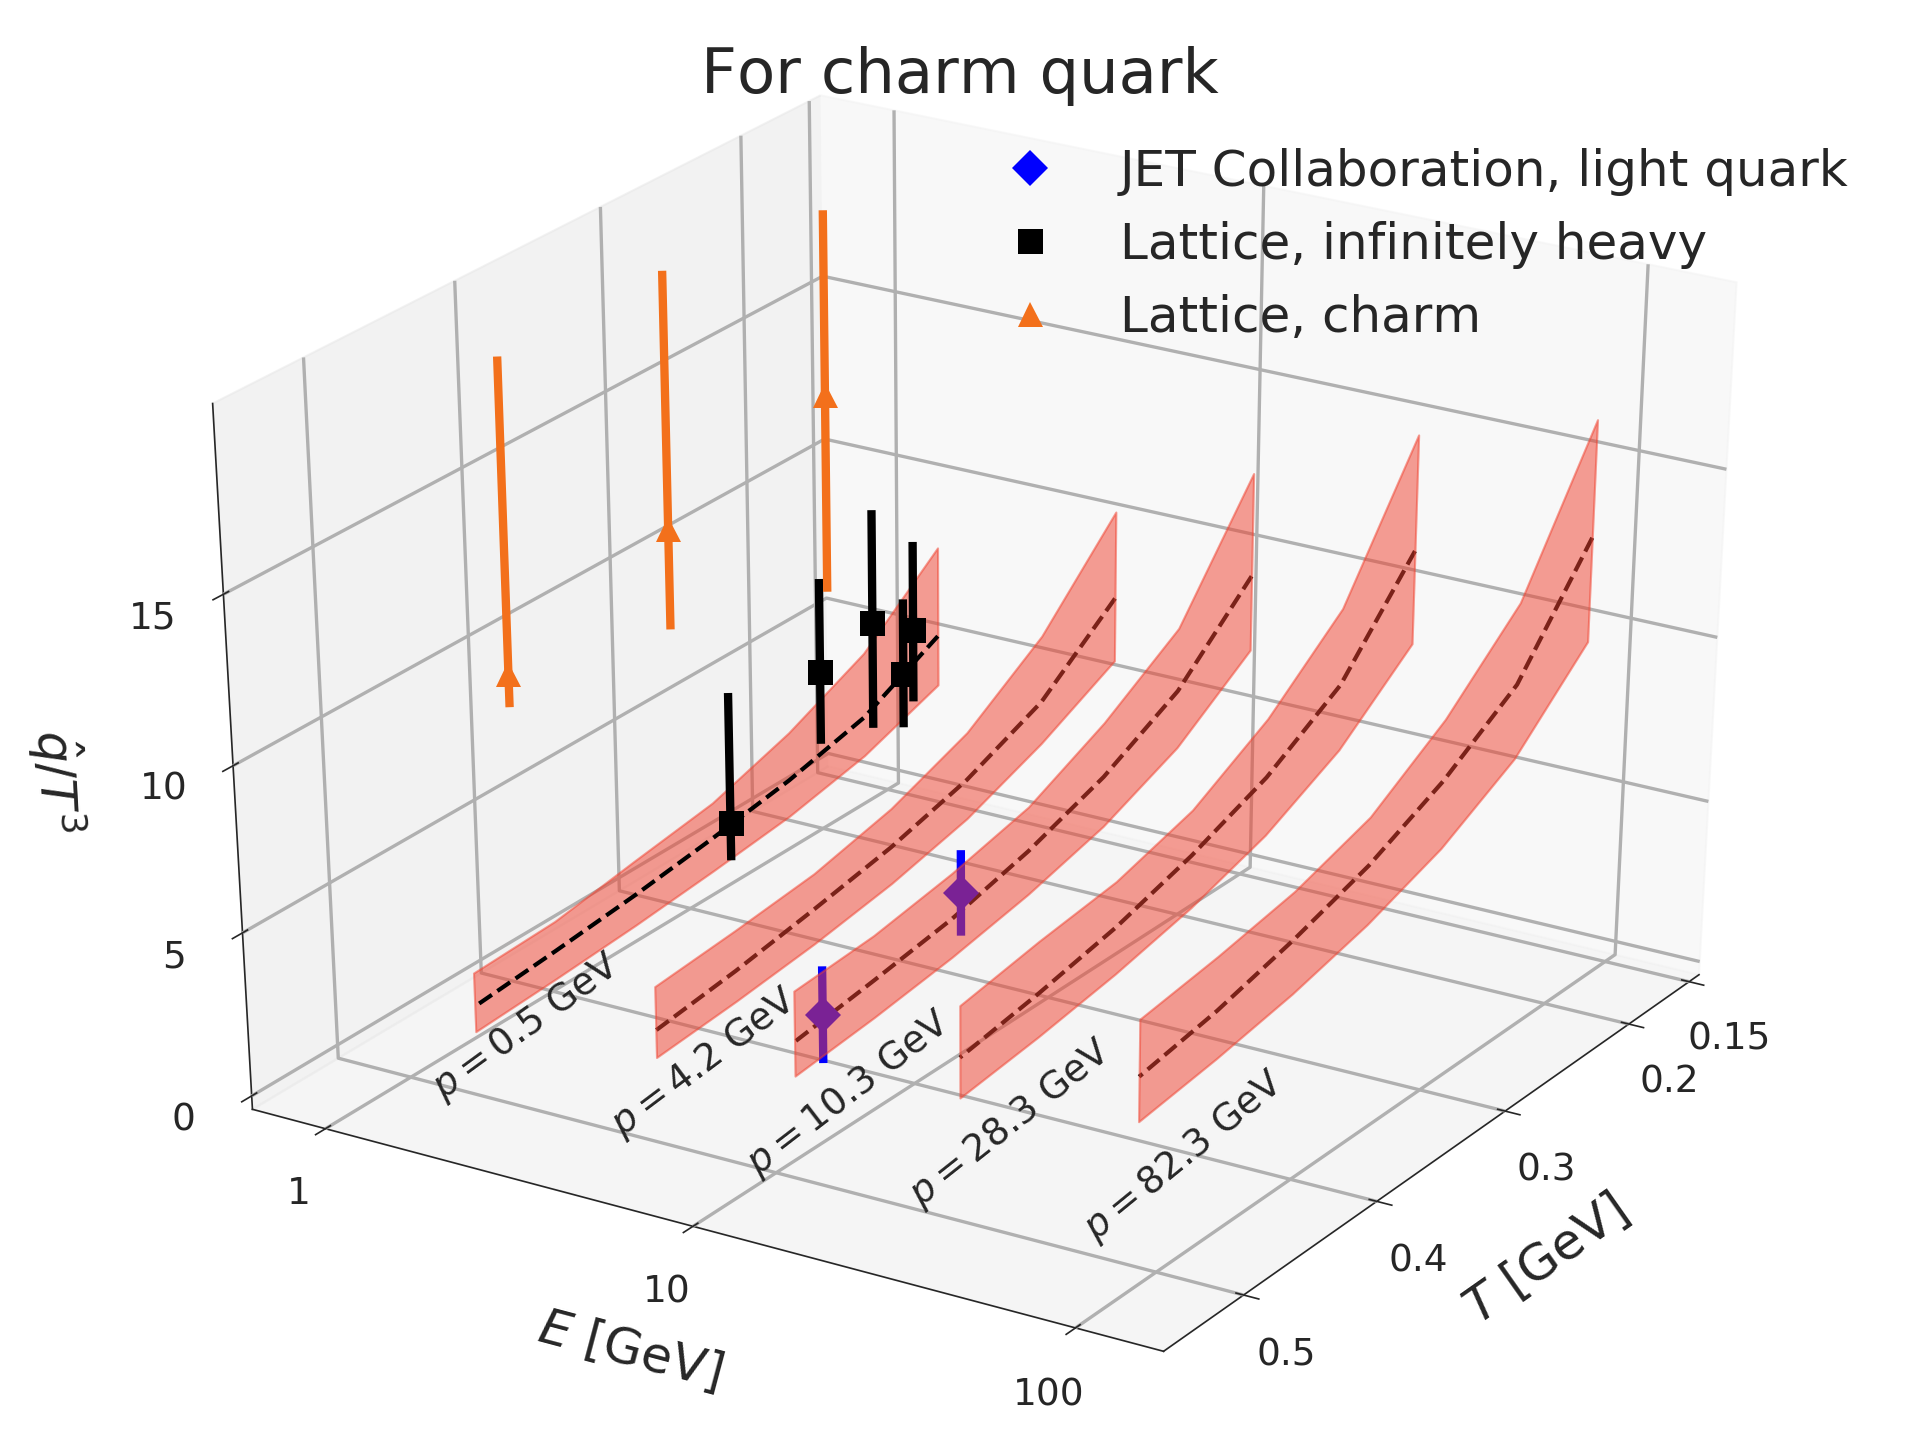
\includegraphics[width=.8\textwidth]{qhat_posterior_3D.png}
\caption[This figure shows the main result of this dissertation. The 90\%]{This figure shows the main result of this dissertation. The 90\% credible transport coefficient $\hat{q}/T^3$ extracted for the charm flavor is displayed on the two-dimensional landscape of energy and temperature. The JET Collaboration extraction of light quark transport coefficients at $p=10$ GeV \cite{Burke:2013yra} (blue diamonds) and two lattice calculations of the momentum diffusion coefficient $\kappa$ ($\hat{q}=2\kappa$) \cite{Ding:2012sp,Banerjee:2011ra} are plotted for comparison.}
\label{fig:conclusion}
\end{figure}

We highlight the progress of this work in the conclusion figure \ref{fig:conclusion}.
It visualizes the $90\%$ credible region of the energy and momentum dependence of the heavy-quark momentum-diffusion transport parameter $\hat{q}$ scaled by $T^3$.
We found $\hat{q}/T^3$ gradually increases with $\ln E$ and displays an enhancement near the critical temperature.
Studying heavy flavor helps to connect the knowledge of in-medium transport properties at very high momentum (light quark limit) and very low momentum (static sources limit).
At relatively high momentum $p\sim 10$ GeV, it is consistent with the light quark transport parameter extracted by the JET Collaboration (blue).
At low momentum, it is consistent with lattice calculations in the heavy quark limit (black).
Future study with improved flavor dependence may be needed to understand the impact of using the ``heavy' limit in a dynamical model.
In the present calibration, the effective in-medium strong coupling constant is about $0.3$ and only contributes to a small fraction of the extracted $\hat{q}$ parameter.
The rest comes from the parametric contribution whose origin can be either perturbative or non-perturbative; either way, it suggests the necessity to model beyond leading order physics.

In conclusion, a transport model with perturbative parton evolution with a parametric probe-medium interaction term provides a reasonable description to the open-heavy flavor observables measured at RHIC and LHC, while the level of accuracy needs to be improved.
Extracted heavy quark transport coefficients as a function of energy and temperature are consistent with early phenomenological studies and lattice calculations.

The present model accuracy is still not enough to make the best use of future high-precision hard probe measurements in heavy-ion collisions.
We, therefore, list a few necessary points of improvements which may help to reduce or estimate the theoretical and modeling uncertainties.
\begin{itemize}
\item An interpolation formula between vacuum and medium-induced radiation: a calculation that connects virtuality evolution with in-medium time evolution will help to eliminate the matching scale uncertainty. Even though its effect is not strong for the present observables and $p_T$ range, it may impact more delicate jet observables.
\item Correlations among multiple emissions in the presence of a medium. We have been neglecting the correlation among subsequent emissions in the ``modified transport model''. In the infinite medium limit, this is because the probability of overlapping emissions scales as $\tau_{1,f} R(\omega_2) \sim \tau_{1,f} \alpha_s/\tau_{2,f}$ which is suppressed by $\alpha_s$. However, this higher-order effect can be important since the phenomenological $\alpha_s$ is not small. There are ongoing studies on this topic \cite{Arnold:2015qya,Arnold:2016kek,Arnold:2016mth,Arnold:2016jnq}.
\item Off equilibrium corrections to the linearized transport equation. One essential assumption in the linearized transport model is that medium partons follow local thermal distributions, even though the hydrodynamics used includes viscous corrections. 
In fact, the viscous correction and the momentum space anisotropy can be huge at early times of the hydrodynamic evolution. 
One needs to understand how these off-equilibrium effects change the interpretation of the transport coefficients one extracts assuming full thermal equilibrium of partons.
\item Dynamical hadronization model and improved treatment of energy loss in the hadronic stage.
Our current hadronization model has the problem of pinching long-distance physics into an instantaneous process. 
At low-$p_T$, the sudden recombination model breaks the detailed balance of the transport model and dynamically treating the recombination process would be desirable.
At high-$p_T$, the problem is more severe, as the large boost dilates the hadronization time. 
Moreover, the hadronic system near $T_c$ is still very dense, and it is inconsistent to apply the vacuum fragmentation function at $T\sim T_c$.
One possible solution for those high-$p_T$ heavy quarks (the recombination process is negligible) is to continue their partonic transport into the hadronic phase, and finally apply the vacuum fragmentation function when the system is dilute enough.
Meanwhile, one can also study the energy loss in the dense hadronic system to extend the extracted transport parameter to the region below $T_c$.
\item A calibration with the simultaneous tuning of the soft and hard sectors. Currently, a separate analysis calibrates the bulk medium evolution. With future high-precision hard-probe measurements, a simultaneous calibration of both soft and hard sector would be interesting.
For example, we find that the number of binary collision as a function of centrality is quite sensitive to the proton shape modeling in the Monte-Carlo Glauber model. 
The sensitivity of hard probe production to the number of binary collisions may help to improve the proton shape modeling in the soft sector. 
In turn, a better-calibrated medium may help to reduce the uncertainty in the hard parton energy loss study.
\end{itemize}
